\documentclass[12pt]{article}
\usepackage[total={18cm,22cm},top=3cm,left=2cm,right=2cm]{geometry}
\parindent=0mm
\usepackage[utf8]{inputenc}

\usepackage{booktabs}

\usepackage[table]{xcolor}

\usepackage{multicol}

\usepackage{graphicx}

\usepackage{amsmath}

\usepackage{tikz}
\usepackage{enumitem}
\definecolor{azulF}{rgb}{.0,.0,.3}
\newcommand{\cnumero}[2]{\tikz[baseline=(myanchor.base)]
\node[minimum size=0.2cm,circle,
inner sep=1pt,draw, #2, thick, fill=#2](myanchor)
{\color{white}\bfseries\fontsize{8}{8}#1};}

\newcommand*{\itembolasazules}[1]{\protect\cnumero{#1}{azulF}}

\usepackage{fancyhdr}
\pagestyle{fancy}
\fancyhf{}
%TODO
\fancyhead[L]{Teoría de Sistemas - Grupo Fénix}
%TODO
\fancyhead[R]{UNAH-VS}
\fancyfoot[C]{\thepage}

\renewcommand*\contentsname{Contenido}

\begin{document}
%*******************************************************
% Portada
%*******************************************************
\begin{titlepage}

  \begin{center}
    {\includegraphics[width=0.65\linewidth]{$HOME/Dev/dotfiles/VimTempls/Imgs/unahvs-logo.png}\par}
  
    {\bfseries\Huge Universidad Nacional Autónoma de\\
                     Honduras en el valle de Sula \par}
  
    \vspace{1cm}
  
%TODO
    {\scshape\huge TEORÍA DE SISTEMAS\par}
  
    \vspace{1cm}
  
%TODO
    {\scshape\Large EJERCICIOS SOBRE DFD DE CONTEXTO}
  
    \vfill 
    {\large Catedrático:\par} %TODO
    {\large Lic. Tania Pineda\par} %TODO
  
    \vfill

      \textbf{\textit{ Grupo Fénix }}
    
      \begin{tabular}{lr} \toprule
          Nombre Completo & No. Cuenta\\ \midrule
          Areli Yaniris Flores Soto & 20172030394 \\
          Paola Maria Pérez Reyes & 20152030878 \\
          Samuel Alejandro Suazo Méndez & 20182000862 \\
          Jimmy Xavier Triminio Hernández & 20122008197 \\
          Luis David Romero Enamorado & 20182001663 \\ \bottomrule
      \end{tabular} 

    \vfill
    {\large SEPTIEMBRE 2021\par} %TODO

  \end{center}

\end{titlepage}

%*******************************************************
% Contenido 
%*******************************************************
\newpage
\tableofcontents

%*******************************************************
% Introducción
%*******************************************************
\newpage
\section{ Introducción }
\vspace{1cm}

\begin{center}
\begin{minipage}{12cm}
En este documento, se presenta el diagrama de la resolución
del ejercicio \#1 el cual su asignado al {\it grupo Fénix }
en donde se solicita la creación de un diagrama de DFD,
el cual significa (\textit {diagrama de flujo de datos}), este
diagrama es muy utilizado para la visualización del procesamiento
de datos o su \textit{ diseño estructurado }. Y este es una práctica
común para un diseñador dibujar un contexto a nivel de estos tipos
de diagramas \textbf{\textit { DFD }}.

\end{minipage}
\end{center}

%*******************************************************
% Objetivos 
%*******************************************************
\newpage
\section{ Objetivos }
\vspace{1cm}

\begin{minipage}{12cm}
\begin{itemize}
  \item Analizar el ejercicio propuesto.
  \item Realizar el diagrama DFD que daría resolución al ejercicio.
\end{itemize}
\end{minipage}


%*******************************************************
% Tema del documento 
%*******************************************************
\newpage
\section{Ejercicio \#1}

\subsubsection{Planteamiento del ejercicio}

\begin{center}
\begin{minipage}{14cm}
Se necesita contar con un sistema que apoye la gestión de ventas 
de una compraventa de automóviles.\\

El sistema debe de registrar los vehículos que ingresan para la venta
lo cual se desea registrar marca, patente, modelo, año, etc. Con las
características del contrato (periodo en venta, comisión a cobrar, etc.).\\

El sistema debe de apoyar también la gestión de cliente, es decir,
mantener clientes preferenciales y clientes normales, y registrar un historial de clientes que ingresen autos buscados por la justicia. \\

Cuanto llega un auto que se requiere vender el sistema se conecta con el
sistema computacional del servicio de Servicio de Registros de Vehículos
Motorizados, en donde determina si el vehículo está libre de litigios 
judiciales o es un vehículo robado. En caso de serlo, debido a numerosos
problemas que ya han ocurrido y han deteriorado la imagen de la empresa,
es que el sistema debiera entregar un aviso automático a la policía de 
Honduras enviándole además un informe con los datos del vehículo
sospechoso.\\

El sistema debiera emitir diversos informes que le sirvan al dueño del 
negocio para verificar el aumento de las ventas, las marcas de autos más
vendidas y de los problemas con autos robados.

\end{minipage}
\end{center}

\vspace{1cm}


\subsubsection{Resolución del ejercicio}

\vspace{2cm}
  \begin{center}
    {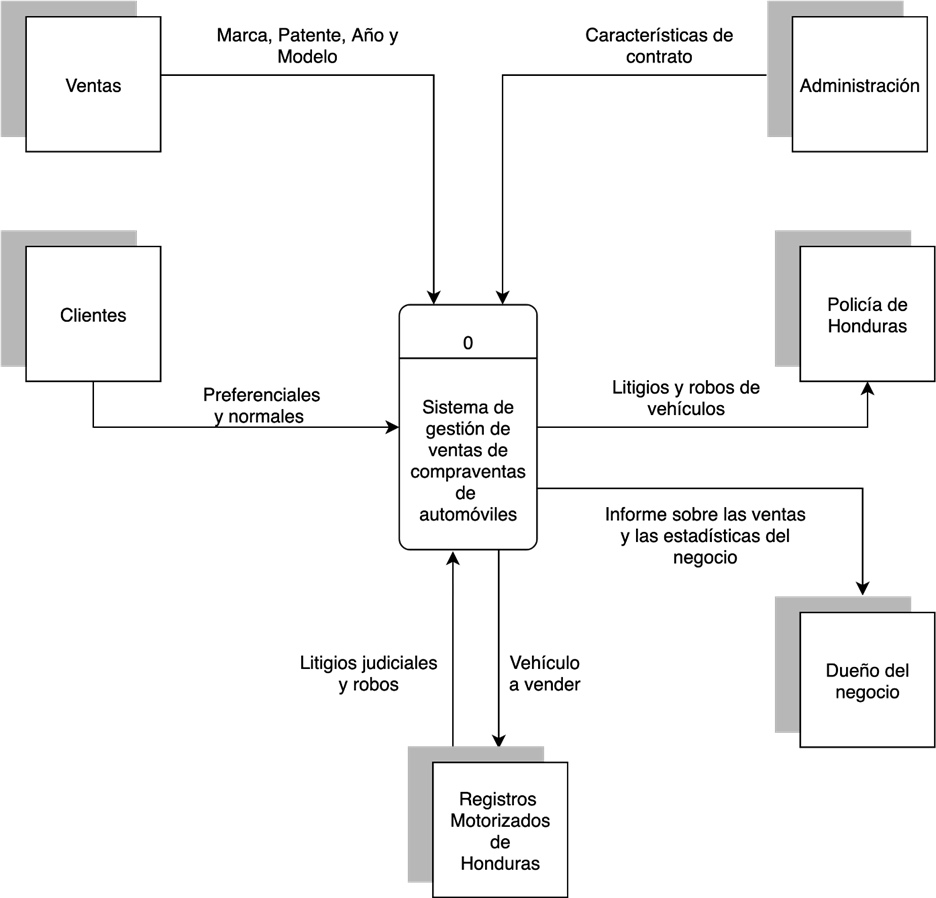
\includegraphics[width=0.85\linewidth]{./DiagramaDFD.png}\par}
  
  \end{center}
%*******************************************************
% Conclusiones 
%*******************************************************
\newpage
\section{ Conclusiones }
\vspace{1cm}

\begin{center}
\begin{minipage}{12cm}
  Realizando la presentación gráfica de flujo de datos \textbf{DFD},
  hemos puestos en practica nuestros diferentes habilidades de trabajo
  en grupo, obteniendo de cada integrante del \textit{grupo Fénix} sus
  opiniones y puntos de vista, y ver los diferentes vías que tomara 
  la resolución de esta actividad. y presentamos nuestra gráfica DFD.
\end{minipage}
\end{center}


%*******************************************************
% Bibliografías 
%*******************************************************
\newpage
\section{ Bibliografías }
\begin{enumerate}
  \item \textit{Wikipedia}\\
    \textit{para la definición del acrónimo} DFD\\
    \textbf{DFD} - {\bf D}iagrama de {\bf F}lujo de {\bf D}atos

\end{enumerate}

\end{document}
end{document}

